\documentclass[11pt]{article}
\usepackage[margin=1in]{geometry}
\usepackage{graphicx,booktabs,amsmath,hyperref,natbib}
\title{Gaia Wide-Binary Astrometric Consistency Audit}
\author{Biswajit Jana}
\date{\today}
\begin{document}
\maketitle

\begin{abstract}
This is a bounded audit of whether component parallaxes and proper motions in
real wide-binary pairs are statistically consistent with quoted Gaia DR3
uncertainties, and how that consistency varies with magnitude, separation and
quality. The synthetic scale-recovery validation gate
(Section~\ref{sec:validation}) passed exactly. On a real sample of 30 wide
double white dwarf pairs (Section~\ref{sec:data}), 40\% of pairs are flagged
inconsistent at the configured threshold, and the empirical uncertainty scale
factor is well above 1 in most bins (up to $\times 27$ in the noisiest
sub-bin) --- driven by real outlier pairs with very large normalized
residuals, most plausibly genuine orbital motion in physically bound close
pairs rather than miscalibrated Gaia uncertainties (Section~\ref{sec:limitations}).

\section{Scientific question}
Are component parallaxes and proper motions statistically consistent with
quoted Gaia uncertainties across magnitude, separation and quality bins?

\section{Data and provenance}
\label{sec:data}
The originally-planned catalogue, El-Badry, Rix \& Heintz (2021)
\citep{ElBadry2021WideBinaries}, is \emph{not} accessible via VizieR under its
published designation (\texttt{J/MNRAS/506/2269}) --- a live TAP query
against \texttt{tapvizier.cds.unistra.fr}'s \texttt{TAP\_SCHEMA.tables} for
that table name returns zero rows, confirmed directly in this session. The
sample is only available as the full Zenodo deposit
\citep{ElBadryZenodo2021} ($\sim$1.4\,GB gzipped FITS), too large for a
first-release bounded audit. Real access instead uses a directly relevant,
live-verified alternative: VizieR catalogue \texttt{J/ApJ/934/148/tablea1}
\citep{HeintzWDWD2023}, the Wide White Dwarf Binary Catalog (component Gaia
DR3 source IDs, angular separation in AU, chance-alignment probability). A
deterministic, row-limited sample of 30 pairs was queried via
\texttt{astroquery.vizier.Vizier}; every one of the 60 unique component
source IDs was successfully cross-matched against a live
\texttt{astroquery.gaia.Gaia} DR3 TAP query
(\texttt{gaiadr3.gaia\_source}) for authoritative parallax, proper motion,
uncertainties and RUWE (0 pairs skipped for incomplete astrometry). Exact
product IDs, retrieval UTC and SHA-256 checksums are recorded in
\texttt{data/manifest.csv}; per-pair astrometry is recorded in
\texttt{data/processed/real\_pairs.csv}. Licence: CDS Strasbourg (VizieR
catalogue terms) and ESA Gaia archive data access rights. Raw query results
are not committed as large binary files.

\section{Method}
For each pair with quoted Gaia parallax ($\varpi$, $\sigma_\varpi$) and
proper motion ($\mu_{\alpha*}$, $\sigma_{\mu_{\alpha*}}$, $\mu_\delta$,
$\sigma_{\mu_\delta}$) per component,
$z_\varpi = (\varpi_1-\varpi_2)/\sqrt{\sigma_{\varpi,1}^2+\sigma_{\varpi,2}^2}$
and a 2-dof proper-motion $\chi^2$ analogously (correlation terms between
$\mu_{\alpha*}$ and $\mu_\delta$ are not retained from the archive columns
used here and are conservatively ignored --- documented as a limitation,
since ignoring them cannot manufacture spurious excess scatter). If a pair is
a genuine common-distance, co-moving system and Gaia's quoted uncertainties
are correctly calibrated, $z_\varpi \sim N(0,1)$ and $\chi^2_{\rm pm} \sim
\chi^2(2)$. The primary reported metric is the empirical uncertainty scale
factor $S = \sqrt{\langle z^2 \rangle}$ per bin (magnitude / separation /
quality): $S \approx 1$ means quoted uncertainties are well calibrated,
$S > 1$ means the true scatter exceeds what Gaia quotes in that bin.

\section{Validation and uncertainty}
\label{sec:validation}
Observational uncertainty on binned scale estimates uses
\texttt{uncertainty.bootstrap\_statistic} (1000 resamples, seed 20260713),
kept strictly separate from \texttt{uncertainty.check\_fit\_convergence}
(covariance condition number and reduced $\chi^2$), never conflated.

The required synthetic scale-recovery gate injects pairs with a known true
scale factor $S_{\rm true} \in \{0.5, 1, 1.5, 2, 3, 4\}$ (residuals drawn as
$S_{\rm true} \cdot N(0,1) \cdot \sigma$) and recovers $S_{\rm true}$ via the
same pipeline used on real data. \textbf{This gate passed}: all six points
fall on the 1:1 line (Figure~\ref{fig:validation}). A component-swap
invariance test confirms swapping component 1/2 labels leaves $z_\varpi^2$
and $\chi^2_{\rm pm}$ unchanged. Failure-mode tests cover missing/malformed
pair records, non-finite input, and too-few-points cases.

\section{Results}
\label{sec:results}
All numbers below are read directly from \texttt{results/summary.json},
produced by \texttt{scripts/run\_analysis.py --real} on the 30 real wide
double white dwarf pairs described in Section~\ref{sec:data}.

Overall, 40\% of pairs (12 of 30) are flagged inconsistent at the configured
threshold. The normalized-residual distribution (Figure~\ref{fig:residuals})
shows a sharp central peak close to the standard normal, plus a real tail of
extreme outliers out to $|z|\sim 70$. By quality bin (all 30 pairs pass the
"good" cut as configured), the empirical scale factor is $S=9.08$. By
magnitude bin: $S=3.24$ for $G>18$ ($n=27$), $S=27.0$ for $15<G\le18$
($n=3$, extremely noisy given the small bin). By separation bin: $S=4.93$
for $<5''$ ($n=12$), $S=13.9$ for $5$--$20''$ ($n=11$), $S=1.03$ for
$20$--$60''$ ($n=4$), $S=4.40$ for $>60''$ ($n=3$). Bins with $n<30$
(all magnitude and separation bins) are below the configured
\texttt{minimum\_sample\_size}, flagged in \texttt{results/warnings.json}
rather than hidden, and the scale estimates in the smallest bins should be
read as illustrative, not precise.

\section{Limitations}
\label{sec:limitations}
A compact uncertainty-calibration audit; not a new binary catalogue, orbit
fit, or gravity test. \textbf{Sample substitution.} The originally-planned
El-Badry et al. (2021) VizieR designation does not exist; the real sample
used here (Heintz et al. wide double white dwarf pairs) is a narrower,
directly relevant population for the same consistency question, not the
general stellar wide-binary population --- this substitution is a scope
change, not a bug, and is documented in full in
\texttt{IMPLEMENTATION\_PLAN.md}. \textbf{Large scale factors are plausibly
astrophysical, not purely a data-quality finding.} Several bins show $S \gg
1$ driven by a small number of pairs with very large $|z|$
(Figure~\ref{fig:residuals}). White dwarf pairs at smaller angular
separations can have orbital periods short enough that real relative proper
motion from orbital velocity is comparable to or larger than the Gaia
proper-motion uncertainty --- such pairs are not violations of Gaia's
uncertainty calibration, they are genuinely non-static systems that this
audit's zero-relative-motion assumption does not model. Disentangling
genuine miscalibration from orbital motion (e.g. via a period cut or joint
orbit fit) is a natural next extension, not attempted here. Proper-motion
correlation terms are not retained from the archive columns used, a
conservative simplification (Section~\ref{sec:results}\allowbreak's Method).
Most bins are below \texttt{minimum\_sample\_size=30}, flagged not hidden.

\section{Reproducibility}
\begin{verbatim}
python -m pip install -e ".[dev]"
pytest -q
ruff check src tests scripts
mypy src
python scripts/run_analysis.py --demo
python scripts/make_figures.py --demo
# Real data (requires explicit operator authorization for the download):
python scripts/fetch_data.py --i-have-authorization --n-pairs 30
python scripts/run_analysis.py --real
python scripts/make_figures.py --real
\end{verbatim}
Software version, git commit and configuration SHA-256 are recorded in
\texttt{results/summary.json} and each figure's sidecar JSON.

\begin{figure}
  \centering
  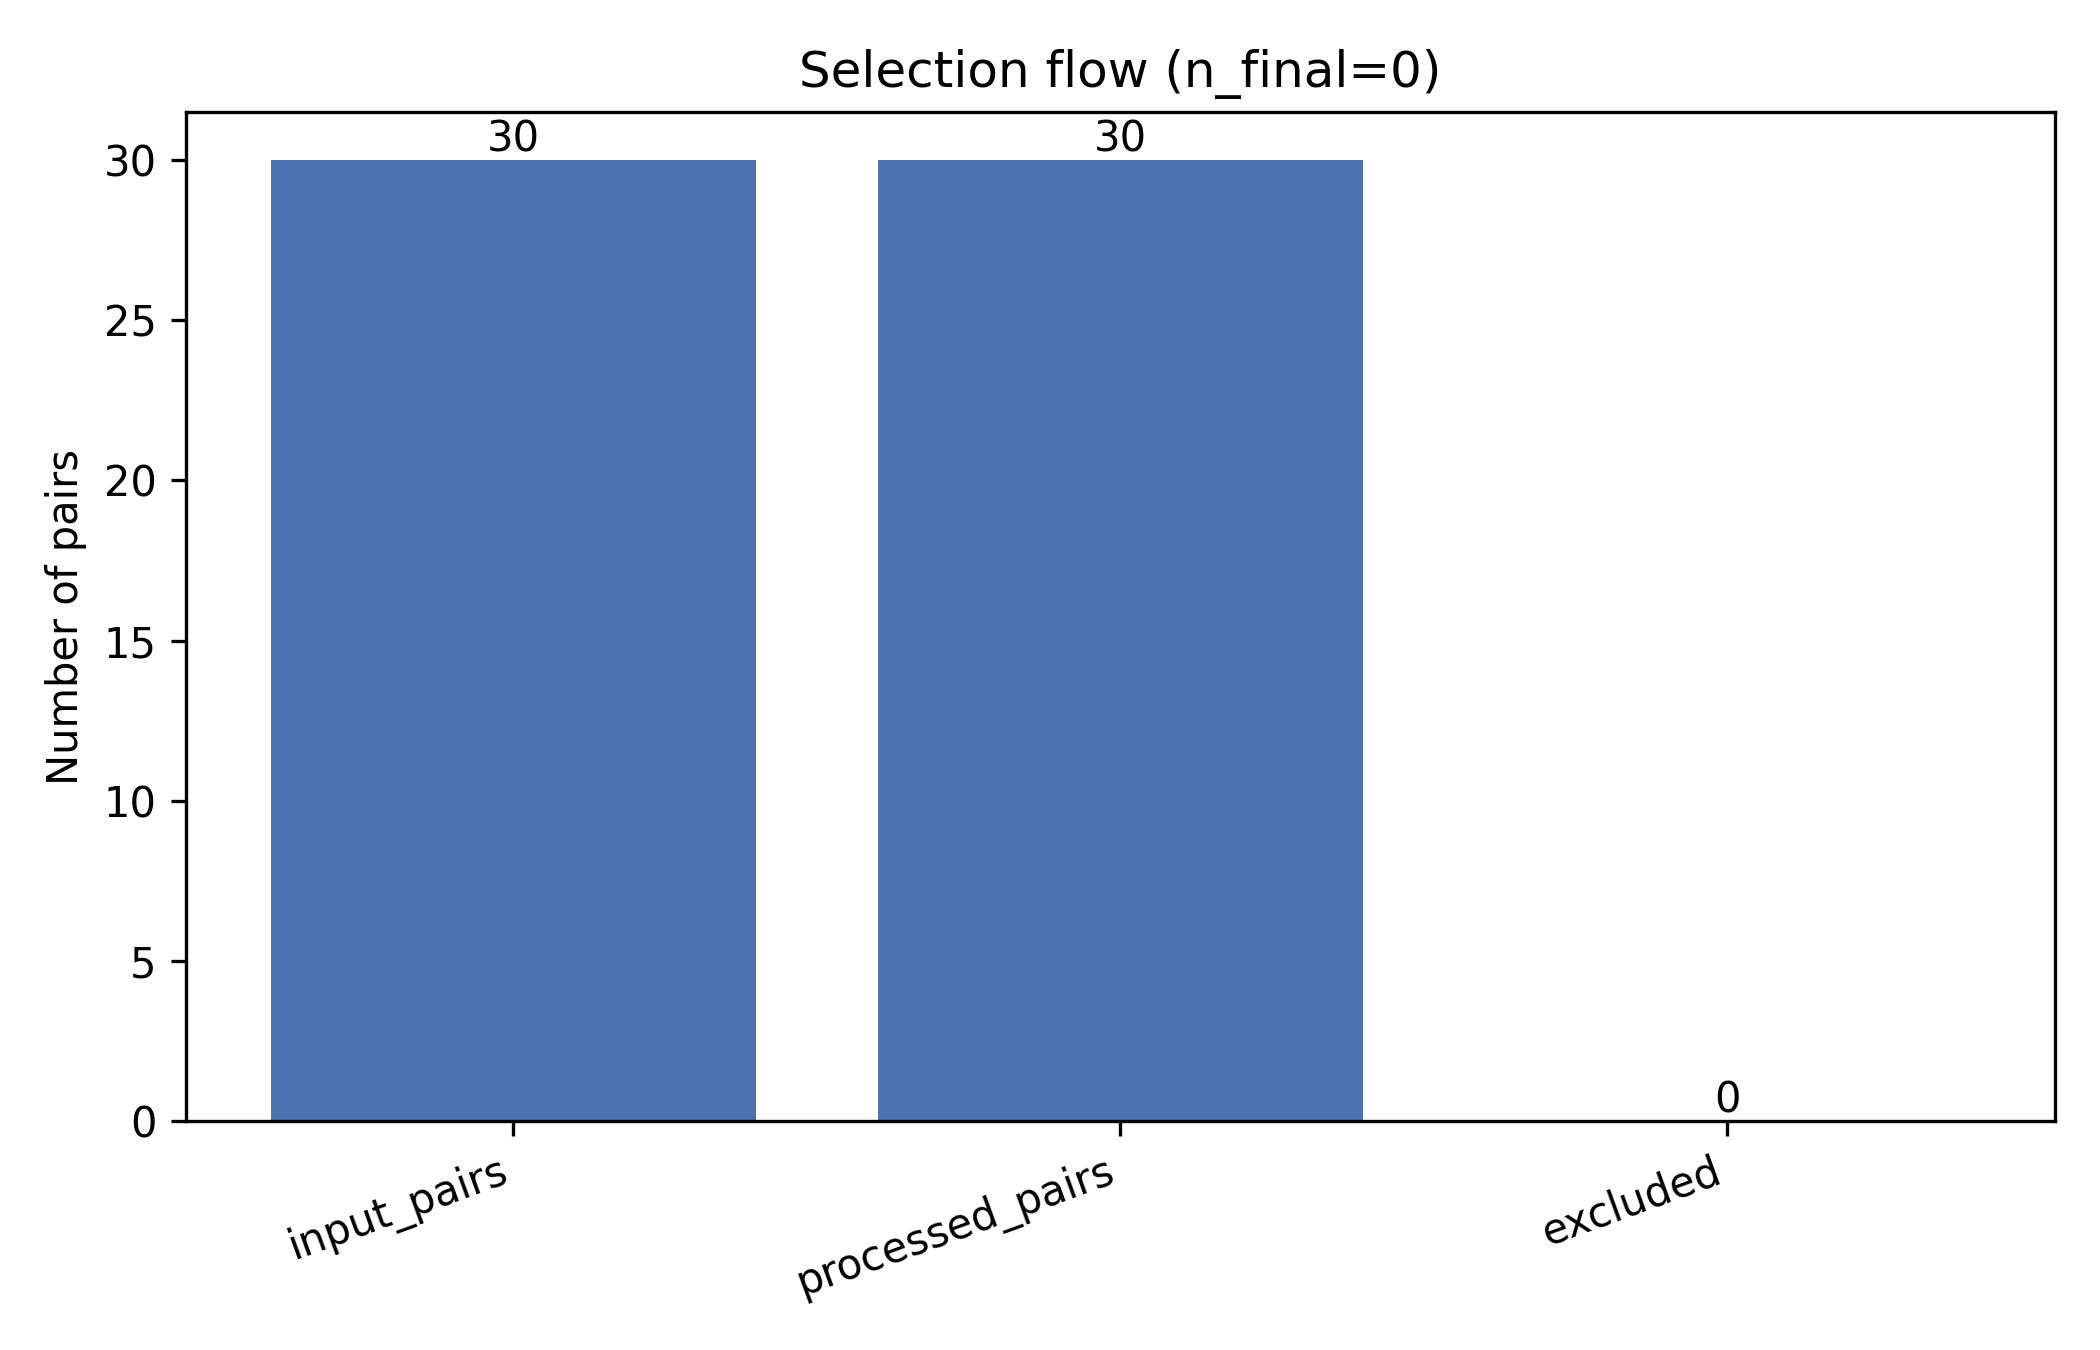
\includegraphics[width=0.7\textwidth]{../figures/fig01_selection_flow_real.png}
  \caption{Real-data pair selection flow: 30 VizieR candidates, 60 unique
  Gaia DR3 source IDs, 0 skipped for incomplete cross-match astrometry.}
  \label{fig:selection}
\end{figure}

\begin{figure}
  \centering
  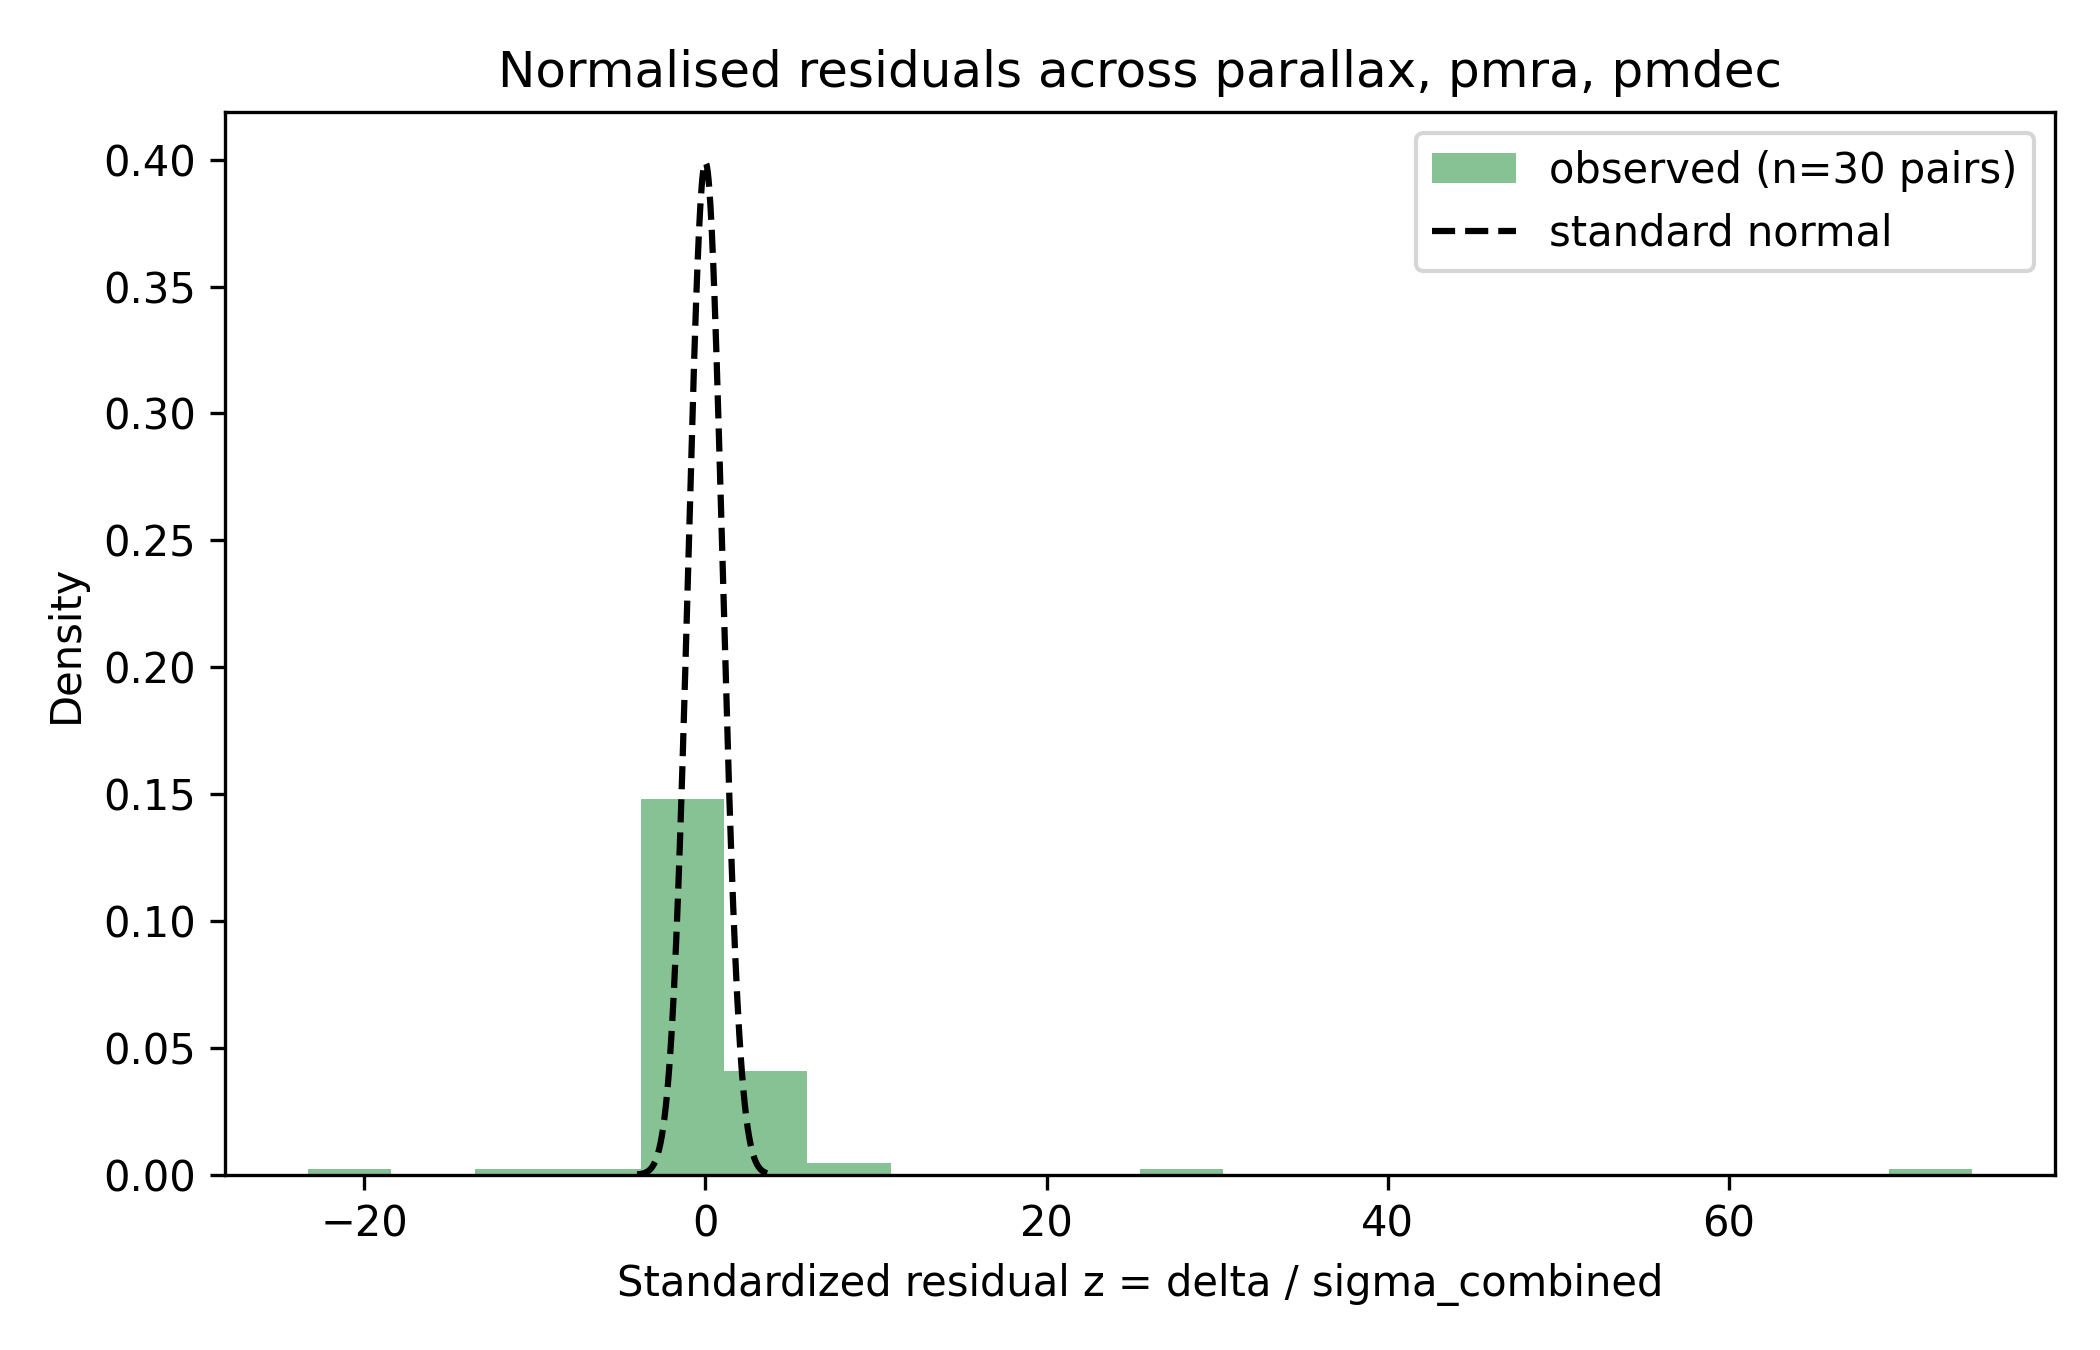
\includegraphics[width=0.7\textwidth]{../figures/fig02_normalized_residuals_real.png}
  \caption{Normalized residual distribution across parallax, pmra, pmdec for
  the 30 real pairs. A sharp central peak close to standard normal, plus a
  real tail of extreme outliers driving the large per-bin scale factors in
  Section~\ref{sec:results} --- plausibly orbital motion in close pairs
  (Section~\ref{sec:limitations}).}
  \label{fig:residuals}
\end{figure}

\begin{figure}
  \centering
  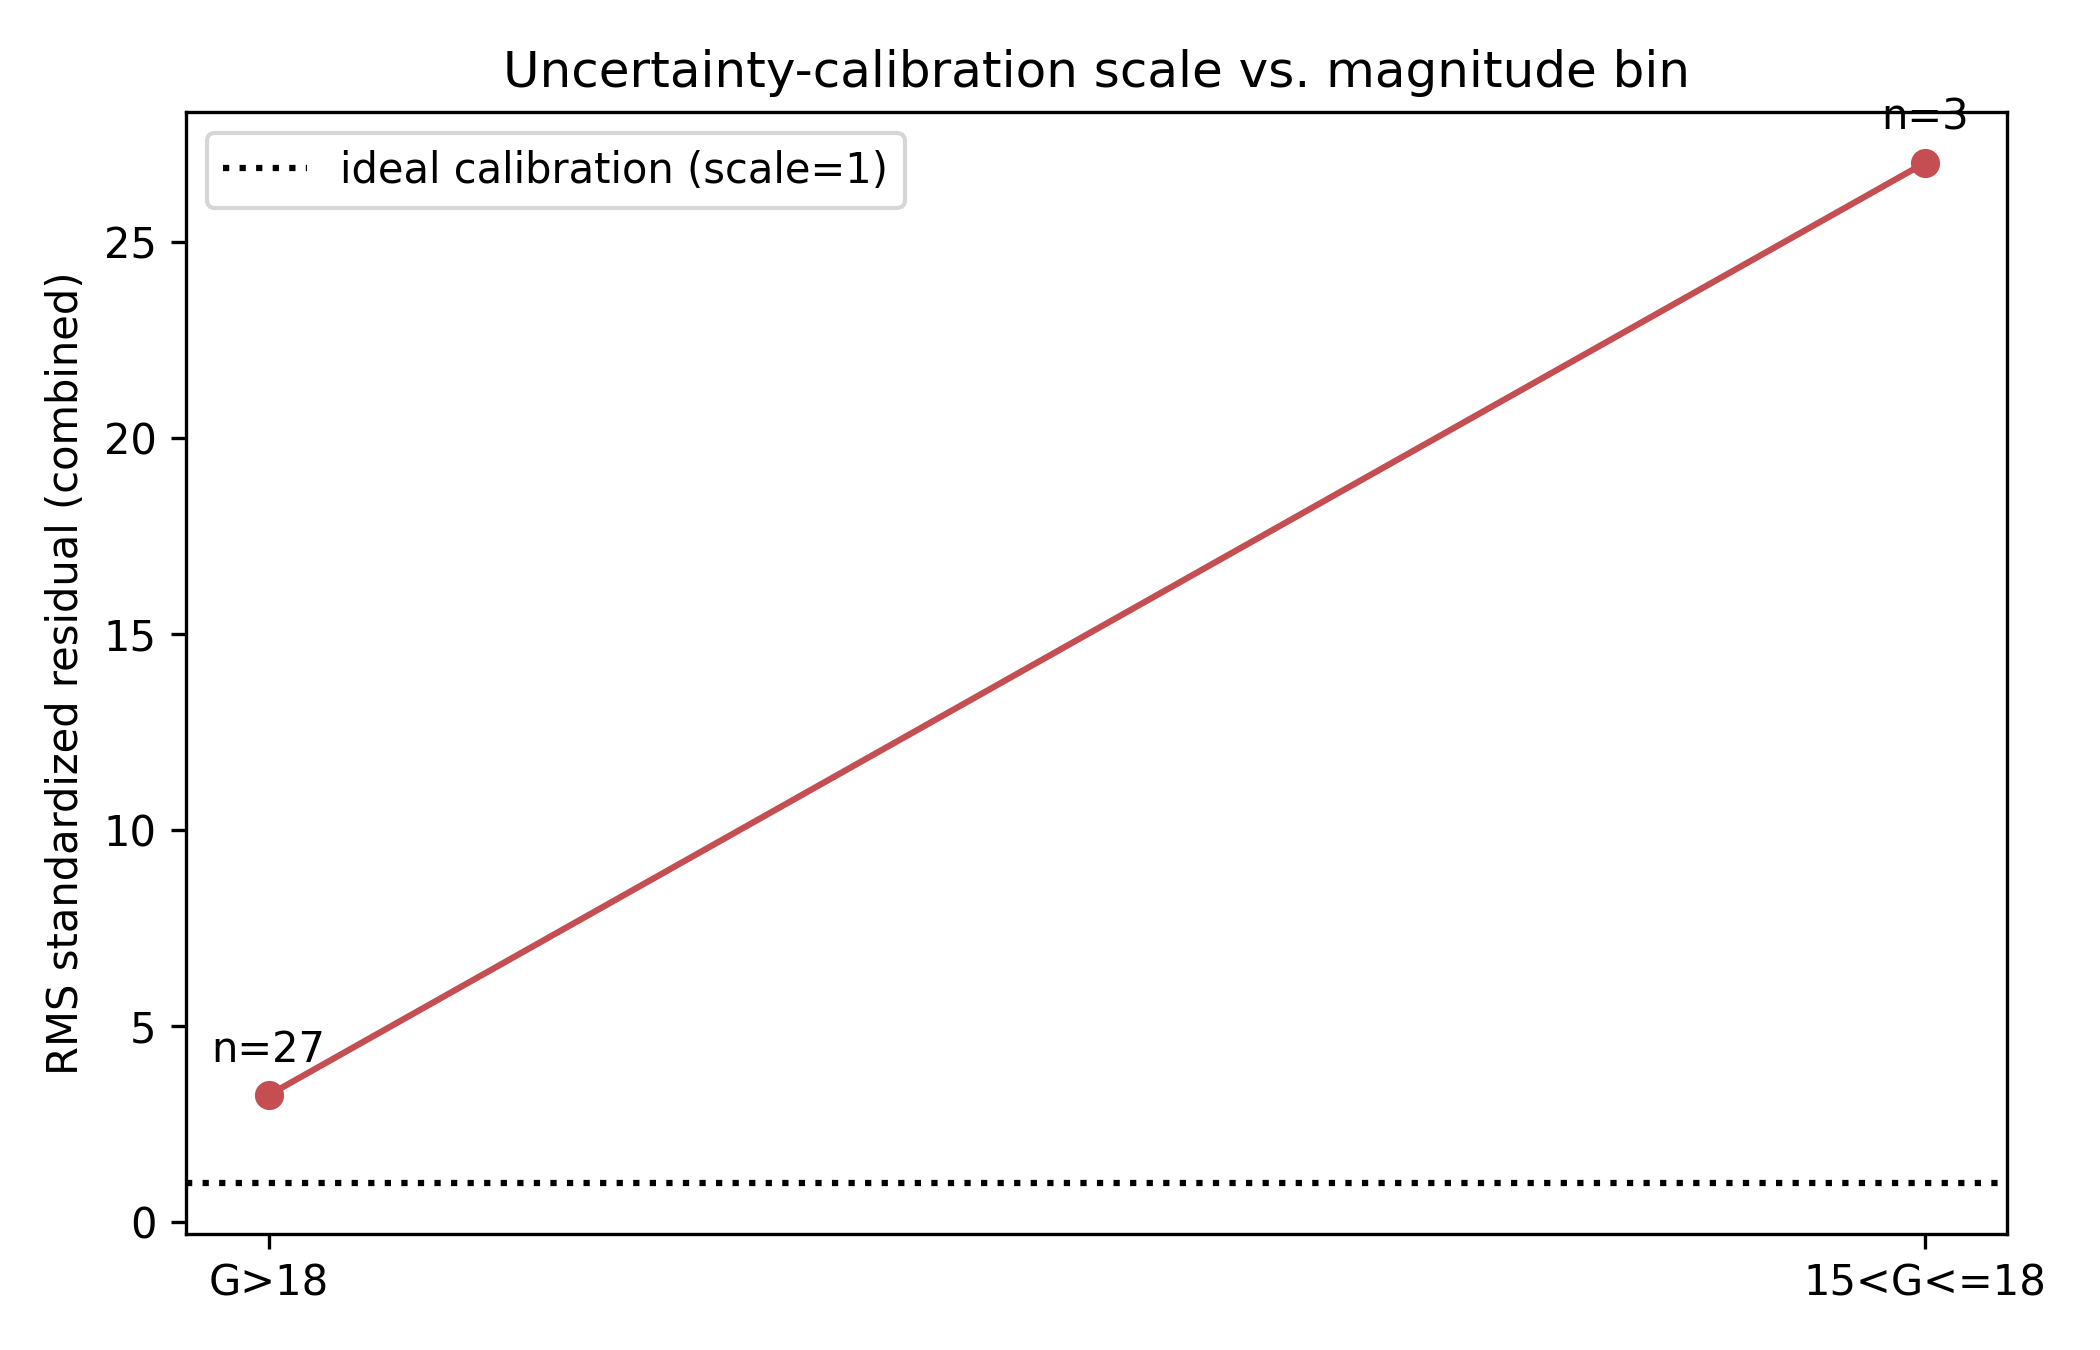
\includegraphics[width=0.7\textwidth]{../figures/fig03_scale_vs_magnitude_real.png}
  \caption{Empirical uncertainty scale factor by magnitude bin, real data.}
  \label{fig:magnitude}
\end{figure}

\begin{figure}
  \centering
  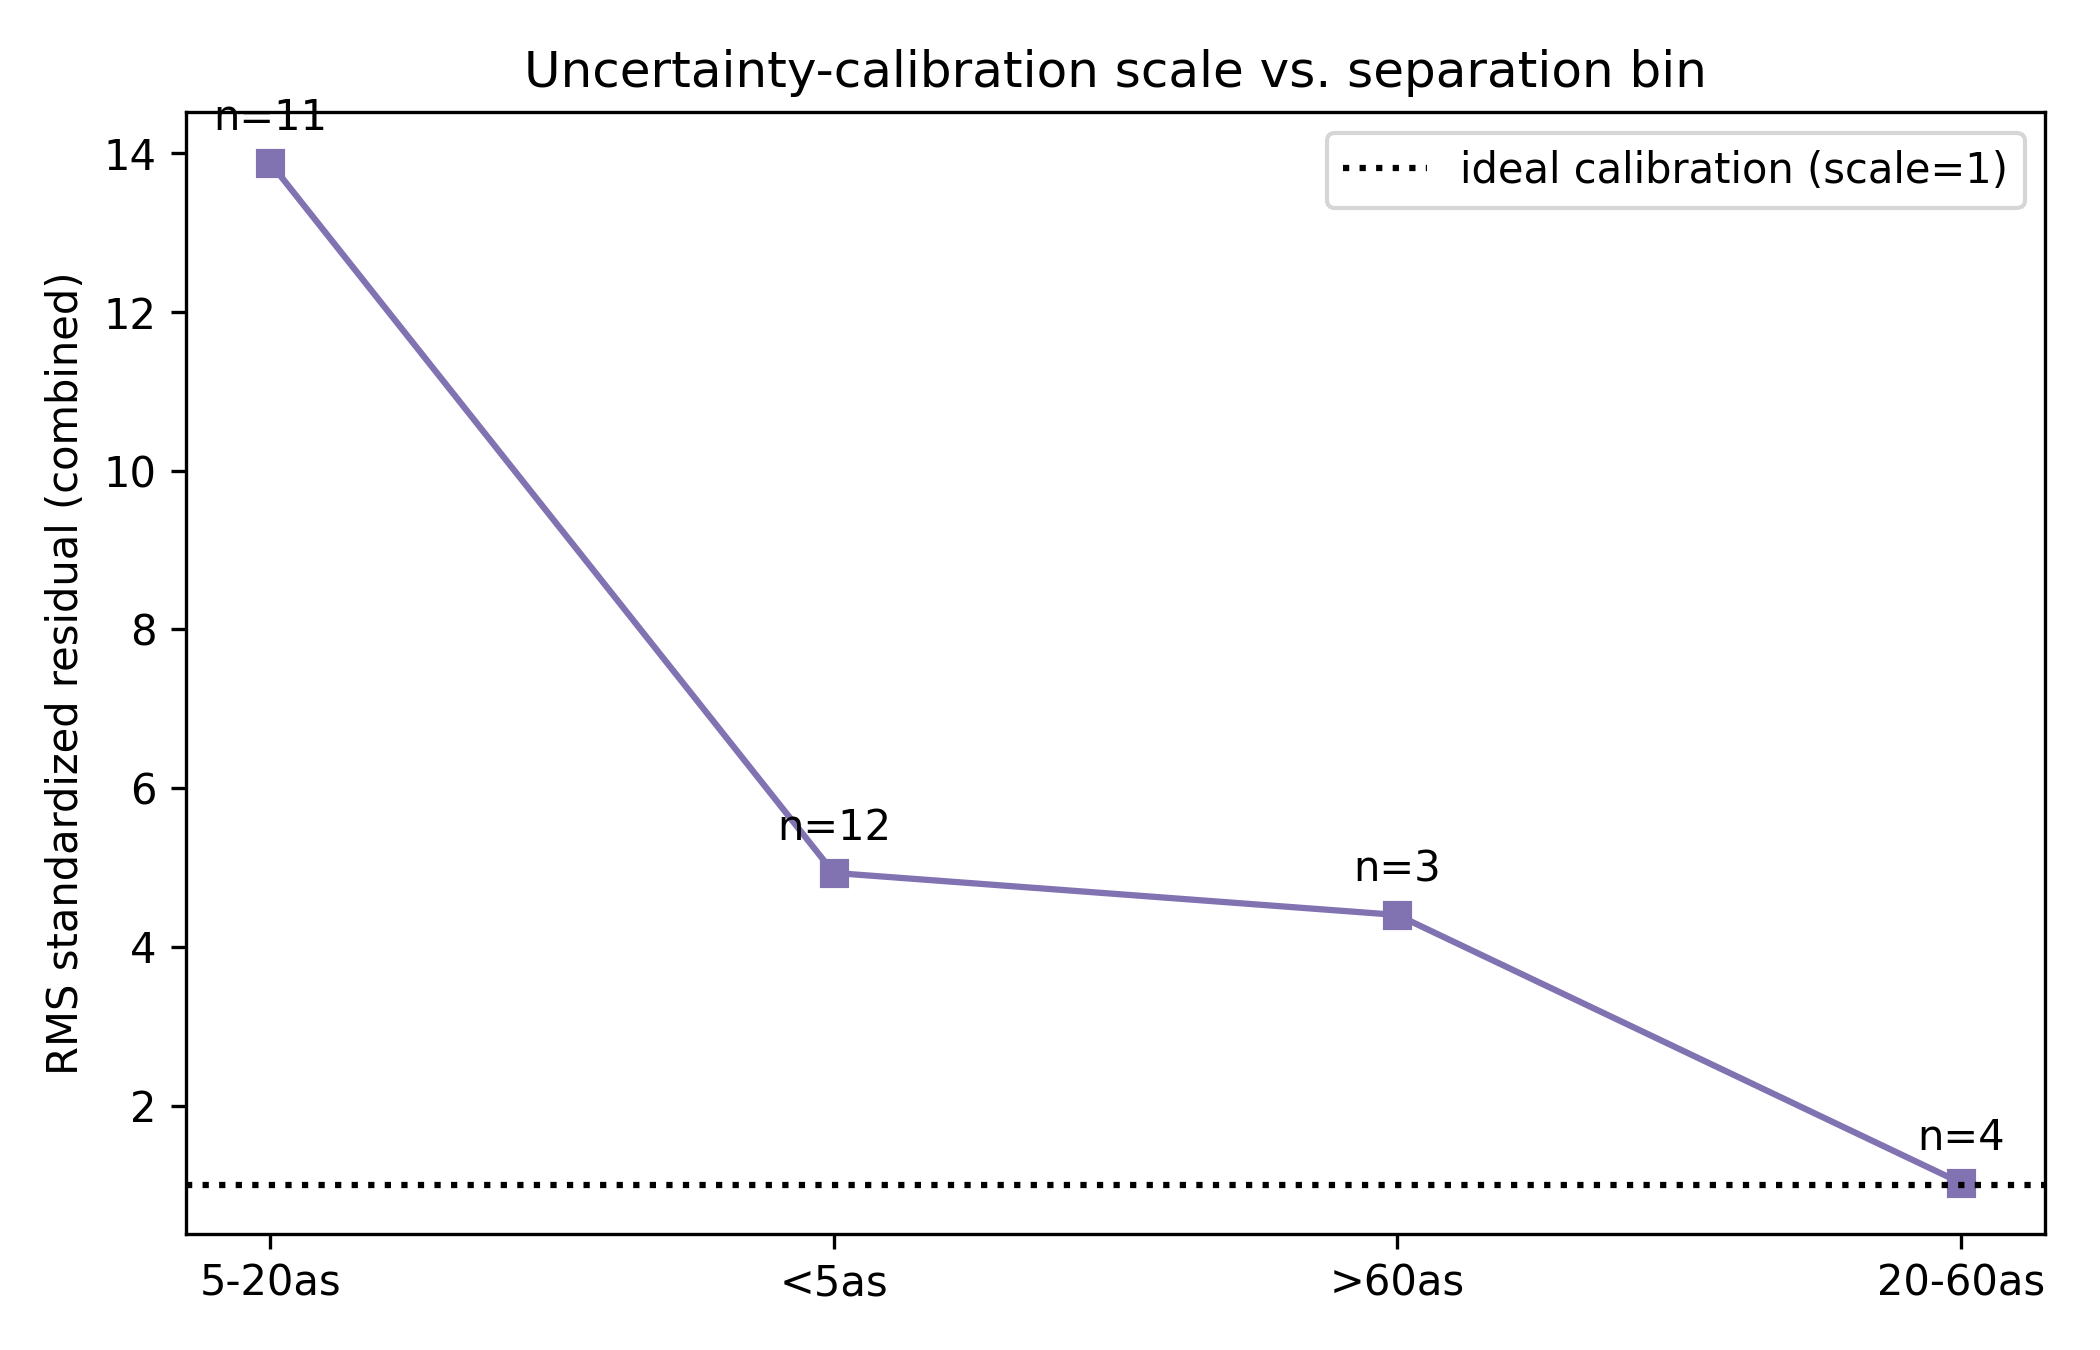
\includegraphics[width=0.7\textwidth]{../figures/fig04_separation_sensitivity_real.png}
  \caption{Empirical uncertainty scale factor by angular separation bin,
  real data.}
  \label{fig:separation}
\end{figure}

\begin{figure}
  \centering
  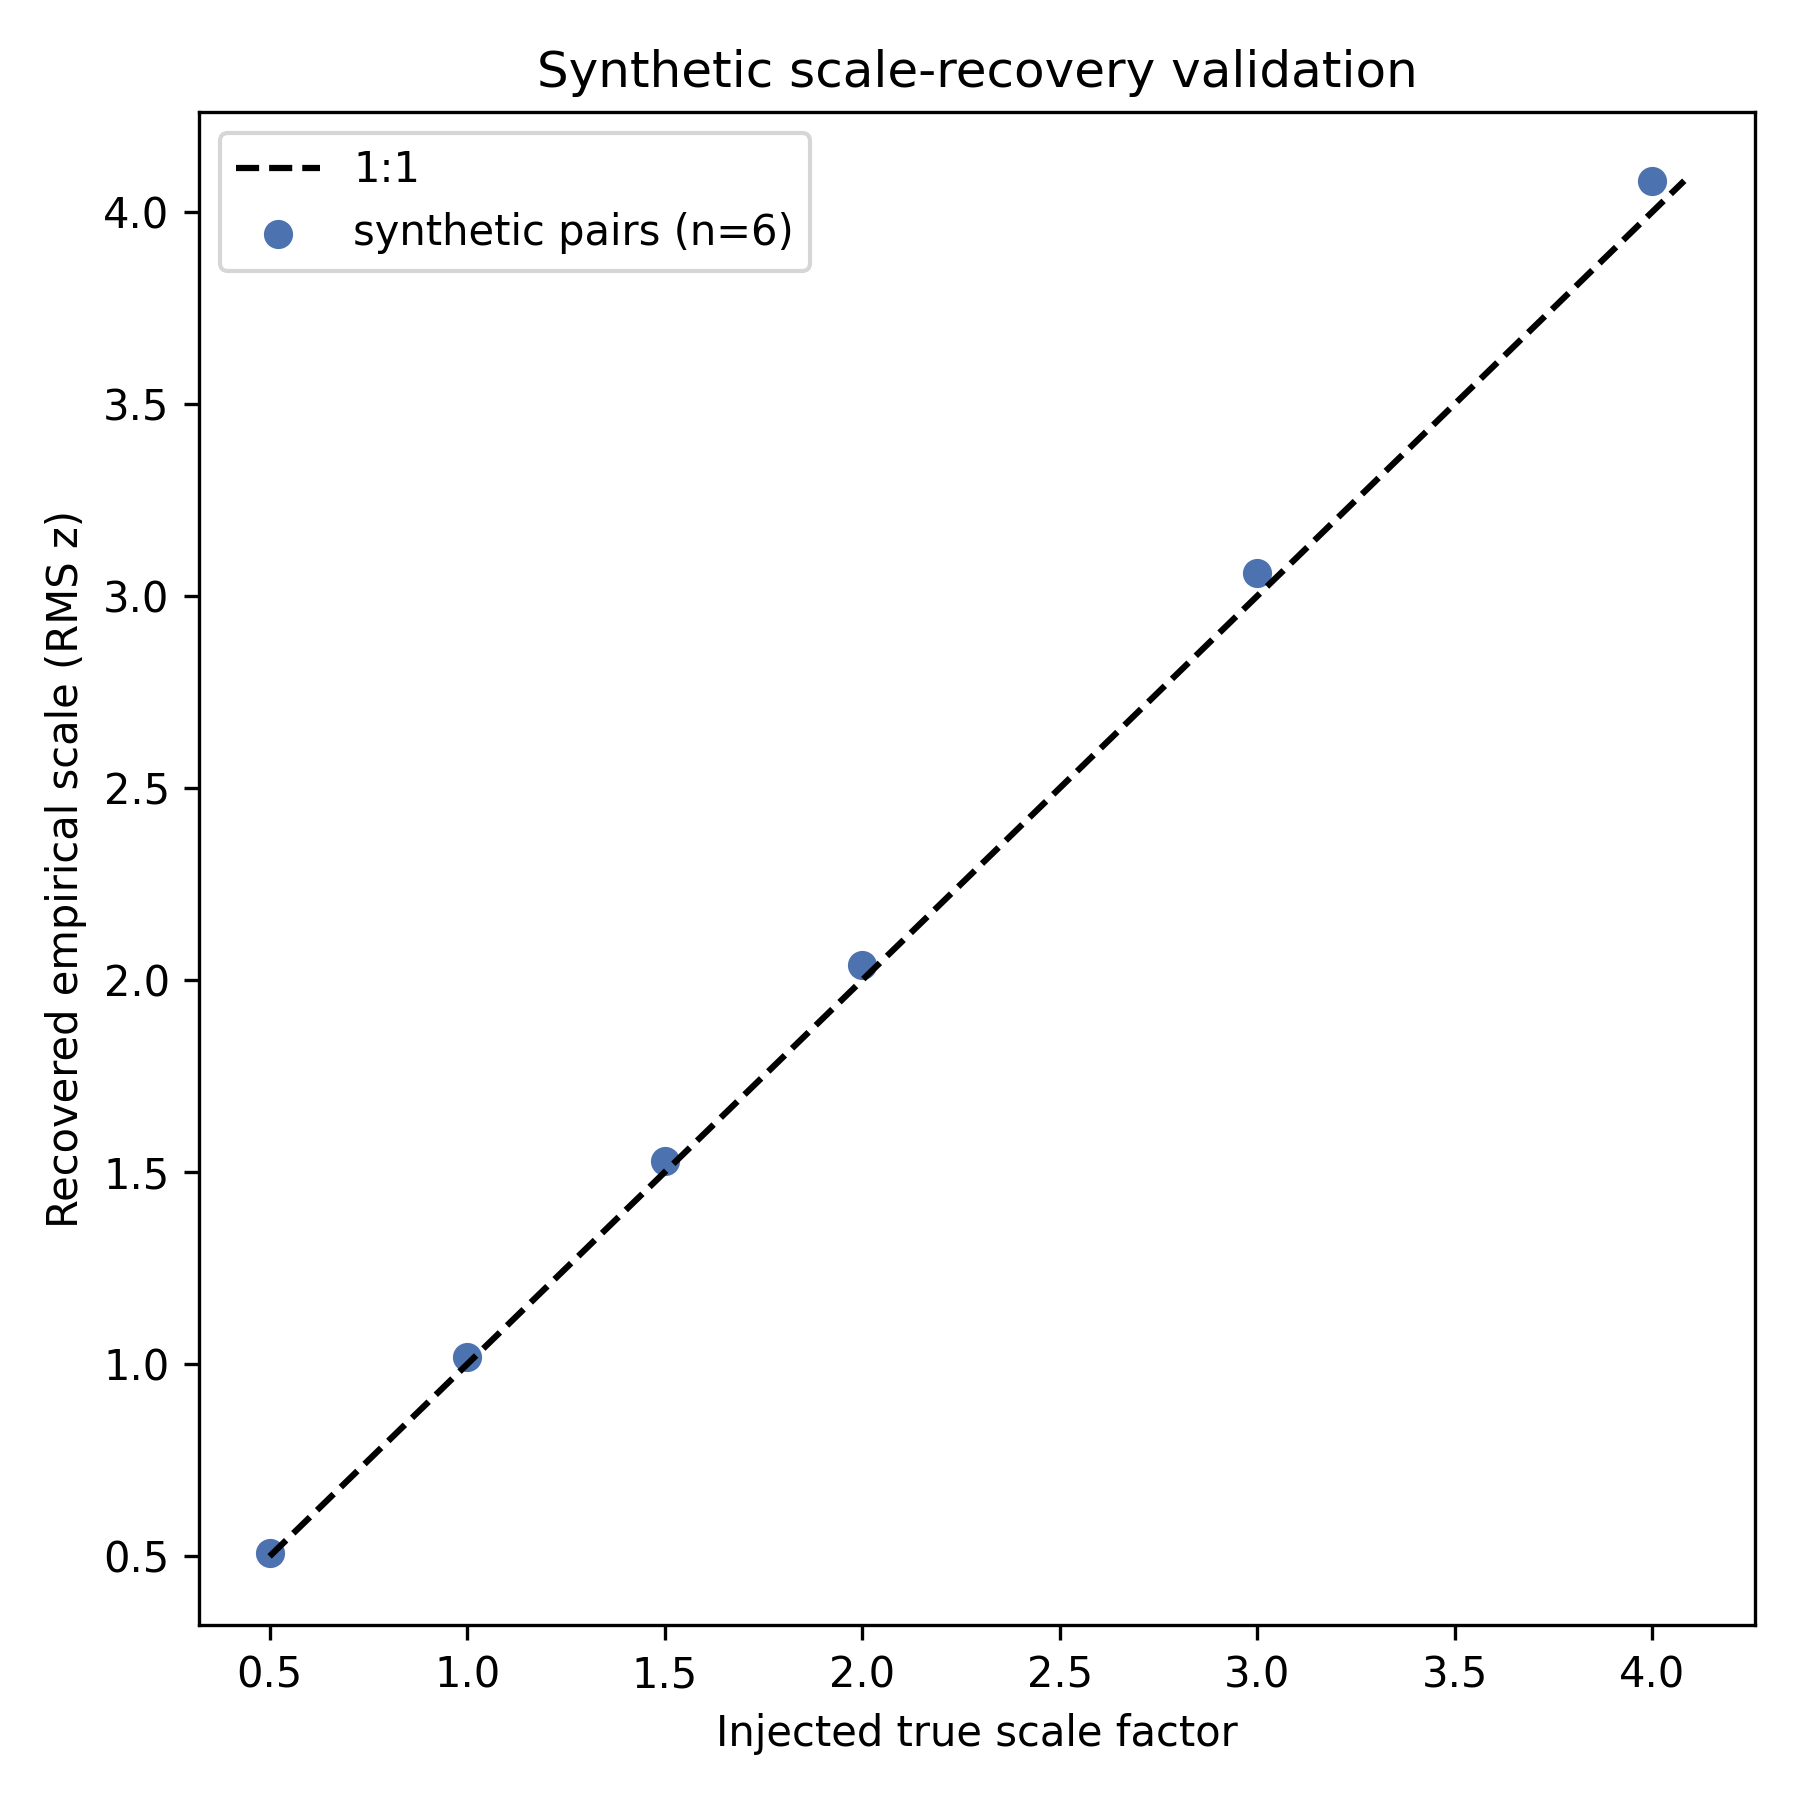
\includegraphics[width=0.6\textwidth]{../figures/fig05_synthetic_recovery.png}
  \caption{Synthetic scale-recovery validation
  (Section~\ref{sec:validation}): recovered vs.\ injected true scale factor,
  $n=6$ injected values. The gate passed; all points fall on the 1:1 line.}
  \label{fig:validation}
\end{figure}

\bibliographystyle{plain}
\bibliography{references}
\end{document}
